\documentclass{"../../res/univ-projet"}
\usepackage[utf8]{inputenc}
\usepackage{array}
\usepackage[T1]{fontenc}
\usepackage[francais]{babel}

\logo{../../res/logo_univ.png}
\title{Spécification Technique des Besoins}
\author{\bsc{Michotte} Maxime}
\projet{M1SSI}
\projdesc{Projet de génération d'OTP}
\filiere{M1SSI}
\version{1.3}
\relecteur{\bsc{Zigh} Benjamin}
\signataire{\bsc{Bardet} Magali}
\date{Décembre 2013}

\histentry{1.3}{15/12/2013}{Ajout des modifications demandées par le client}
\histentry{1.2}{04/12/2013}{Ajout des exigences correspondant au CdR}
\histentry{1.1}{28/11/2013}{Ajout terminologie et modification schémas}
\histentry{1.0}{15/11/2013}{Version initiale.}


\begin{document}
\maketitle
%-------------------------------------------------------------------------------
\section{Objet}
Étude et implémentations des systèmes d'authentification utilisant des mots de passe jetables.

    \subsection{Besoins opérationnels} 
        \begin{itemize}
            \item Garantir une authentification forte.
            \item État de l'art sur les systèmes existants.
            \item Objectif : mise en production.
        \end{itemize}
    \subsection{Objectifs techniques}
    \begin{itemize}	
            \item Implémentation des solutions retenues sur un ou plusieurs supports.
    \end{itemize}
    \subsection{Contraintes et recommandations} 
        \begin{itemize}
            \item Respecter les spécifications de base et les normes RFC.
            \item Montrer que le système produit est sûr.
            \item Choisir une implémentation adaptée en fonction des besoins et de l'état de l'art établi.
        \end{itemize}
    \subsection{Résultats attendus} 
        \begin{itemize}
            \item Système sûr et fonctionnel.
            \item État de l'art le plus exhaustif possible.
            \item Implémentation sur Carte à puces et/ou Android.
        \end{itemize}
        
\newpage
%-------------------------------------------------------------------------------
\section{Documents applicables et de référence}

\begin{tabular}{p{1,5cm}>{\raggedright\arraybackslash}p{13cm}}
{[ANS10]} & {ANSSI. Référentiel général de sécurité. \href{http://www.ssi.gouv.fr/fr/reglementation-ssi/referentiel-general-de-securite}{http://www.ssi.gouv.fr/fr/reglementation-ssi/referentiel-general-de-securite}, 2010.}
\tabularnewline
\\
{[MvOV97]} & {Alfred J. Menezes, Paul C. van Oorschot, and Scott A. Vanstone. Handbook of applied cryptography. CRC Press Series on Discrete Mathematics and its Applications. CRC Press, Boca Raton, FL, 1997. With a foreword by Ronald L.Rivest.}
\tabularnewline
\\
{[RFC98]} & {A One-Time Password System. \href{http://tools.ietf.org/html/rfc2289}{http://tools.ietf.org/html/rfc2289}, 1998.}
\tabularnewline
\\
{[RFC05]} & {HOTP:An HMAC-Based One-Time Password Algorithm \href{http://tools.ietf.org/html/rfc4226}{http://tools.ietf.org/html/rfc4226}, 2005.}
\tabularnewline
\\
{[RFC06]} & {Generic Message Exchange Authentication for the Securer Shell Protocol (SSH).\href{http://tools.ietf.org/html/rfc4256}{http://tools.ietf.org/html/rfc4256}, 2006.}
\tabularnewline
\\
{[RFC07]} & {The EAP Protected One-Time Password Protocol (EAP-POTP). \href{http://tools.ietf.org/html/rfc4793}{http://tools.ietf.org/html/rfc4793}, 2007.}
\tabularnewline
\\
{[RFC11]} & {TOTP: Time-Based One-Time Password Algorithm \href{http://tools.ietf.org/html/rfc6238}{http://tools.ietf.org/html/rfc6238}, 2011.}
\tabularnewline
\\
{[goo]} & {Google Authentificator \href{https://code.google.com/p/google-authenticator/}{https://code.google.com/p/google-authenticator/}.}
\tabularnewline
\\
\end{tabular}

%-------------------------------------------------------------------------------
\section{Exigences fonctionnelles}
\begin{tabular}{|c|l|l|c|}
    \hline
    \rowcolor{gray}
    \textcolor{white}{Id} & \textcolor{white}{Intitulé} & \textcolor{white}{Acteur(s)} & \textcolor{white}{Priorité}\\
    \hline
    EF\_01 & État de l'art & Équipe & Indispensable\\
    \hline
    EF\_02 & Association serveur-client-token & Utilisateur & Indispensable\\
    \hline
    EF\_03 & Génération de l'OTP par le token & Utilisateur & Indispensable\\
    \hline
    EF\_04 & Authentification & Utilisateur & Indispensable\\
    \hline
    EF\_05 & Re-synchronisation & Utilisateur & Indispensable\\
    \hline
\end{tabular}\

\begin{figure}[h]
  \centering
  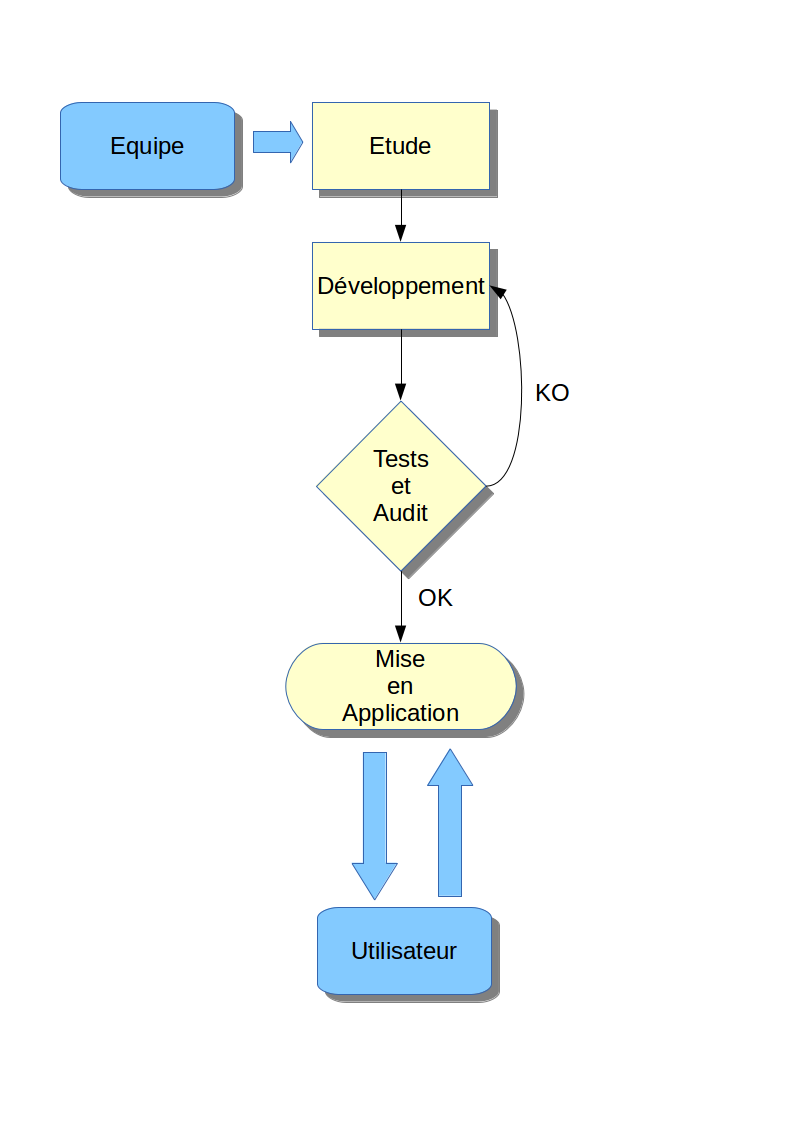
\includegraphics[scale=0.5]{../graphics/diagramme1.png}
  \caption{Schéma Macroscopique du Projet}
  \setlength{\parindent}{1cm}
  \begin{flushleft}
  Nous (l'équipe) commencerons  par une étude des différents protocoles de générations d'OTP afin d'en fournir un état de l'art le plus exhaustif possible. Une fois celui-ci terminé nous passerons \`{a} l'implémentation des meilleurs protocoles retenus. Enfin, pour vérifier notre production, un audit sera organisé ainsi qu'une batterie de tests afin de corriger les erreurs de développement pour nous mener \`{a} une mise en application. 
  \end{flushleft}
\end{figure}




\clearpage

\fiche{Association serveur-client-token}{Utilisateur}{Le serveur communique au Token un secret}{Il existe une communication client-serveur}{Bouton utilisateur}{Association réussie}{../graphics/association.jpg}{Impossible d'associer le token au serveur}
\\

\fiche{Génération de l'OTP par le token}{Utilisateur}{L'utilisateur demande au token un nouvel OTP qui lui est retourné}{Le token est lié au serveur}{L'utilisateur demande un OTP}{OTP généré}{../graphics/generation.jpg}{Null}
\\

\fiche{Authentification}{Utilisateur}{L'utilisateur tente de s'authentifier sur le serveur}{L'utilisateur possède un OTP}{L'utilisateur donne le mot de passe au serveur}{Utilisateur authentifié ou rejeté}{../graphics/authentification.jpg}{Crash du serveur}
\\

\fiche{Re-Synchronisation}{Utilisateur}{Mise en accord du token et du serveur}{Il existe une connexion entre le token et le serveur}{Perte de la synchronisation}{Synchronisation retrouvé}{../graphics/resynchronisation.jpg}{Ne peut pas re-synchroniser}
\clearpage
\newpage
%-------------------------------------------------------------------------------
\section{Exigences opérationnelles}
\begin{tabular}{|c|l|c|}
    \hline
    \rowcolor{gray}
    \textcolor{white}{Id} & \textcolor{white}{Intitulé} & \textcolor{white}{Priorité}\\
    \hline
    EP\_01 & Le Token renvoie un OTP & Indispensable\\
    \hline
    EP\_02 & L'OTP est utilisable 1 seule fois & Indispensable\\
    \hline
    EP\_03 & L'OTP est non prévisible (OTP qui ne peut être déduit des anciens générés) & Indispensable\\
    \hline
    EP\_04 & Résistant à une attaque exhaustive & Indispensable\\
    \hline
    EP\_05 & Résistant aux attaques par rejeu & Indispensable\\
    EP\_06 & Respect des RFC (RFC2289, RFC4226, RFC4256, RFC4793, RFC6238) & Indispensable\\
    \hline

    \hline
    
    
\end{tabular}

%-------------------------------------------------------------------------------
\section{Exigences d'interface}
\begin{tabular}{|c|l|c|}
    \hline
    \rowcolor{gray}
    \textcolor{white}{Id} & \textcolor{white}{Intitulé} & \textcolor{white}{Priorité}\\
    \hline
    EI\_01 & UNIX(Client/Serveur/Token) & Indispensable\\
    \hline
    EI\_02 & Android(Token) & Indispensable\\
    \hline
    EI\_03 & Java Card (Token) & Facultatif\\
    \hline
\end{tabular}

%-------------------------------------------------------------------------------
\section{Exigences de qualité}
\begin{tabular}{|c|l|}
    \hline
    \rowcolor{gray}
    \textcolor{white}{Id} & \textcolor{white}{Intitulé}\\
    \hline
    EQ\_01 & Génération de mots de passe inférieur à 1 seconde (sur un processeur cadencé à 700MHz)\\
    \hline
    EQ\_02 & Temps de réponse serveur (temps < 1 sec + 2 * tps communication)\\
    \hline
    EQ\_03 & Le serveur supporte au moins 100 000 demandes de vérification simultanées\\
    \hline
    EQ\_04 & La vérification est cohérente\\
    \hline
    EQ\_05 & La génération utilise au plus 10 Ko de mémoire\\
    \hline
    EQ\_06 & état de l'art exhaustif, au moins trois protocoles OTP  étudiés\\
    \hline
\end{tabular}
%-------------------------------------------------------------------------------
\end{document}
